\section{PPLT Installieren}
	Die Installation der PPLT gestaltet sich nach Betriebssystem unterschiedlich.
	F�r Posix Systeme empfiehlt es sich die Quellen herunter zu laden. F�r Windows
	existiert ein grafische Installer. Bitte laden sie sich zun�chst die aktuelle
	Version der PPLT von der URL \href{http://pplt.berlios.de}{pplt.berlios.de}
	herunter. Bitte vergessen sie nicht die Module\footnote{Ein ZIP Archiv mit
	dem Name \texttt{Modules-0.2.0.zip}} der PPLT herunter zu laden. In diesem 
	Archiv sind alle Kernmodule sowie die Server und Gr�tedateien enthalten.
	
	\subsection{Installation unter Windows}
	Die Installation der PPLT gestaltet sich durch den Installer recht einfach.
	Sie k�nnen alternativ auch die Quellen herunterladen und diese nach der im
	Abschnitt "`Installation unter Posix"' gegebenen Anleitung Installieren.
	
	F�hren sie also den Installer aus und folgen den Anweisungen im Dialog.
	Meist k�nnen sie die Standardwerte �bernehmen. Ist die Installation
	abgeschlossen, sollten sie noch eine Verkn�pfung auf das PPLT-Center
	(PPLTC.py) herstellen, um dieses einfacher erreichen zu k�nnen. Der
	Installer legt leider keine Verkn�pfung im Startmenu an. Diese m�ssen
	sie mit Hand herstellen, wenn sie das wollen. 
	
	Erzeugen sie zun�chst eine Verkn�fung auf dem Dektop imdem sie das Kontextmen�
	mit der rechten Maustaste �ffnen. Klicken sie dann auf \texttt{Neu->Verkn�pfung}
	und dann im sich �ffnenden Fenster auf \texttt{Durchsuchen}. Gehen sie in das 
	Verzeichnis, in das sie Python installiert haben. Dort findet sich ein Ordner
	mit dem Namen \texttt{Scripts} in diesem Ordner liegt die Datei \texttt{PPLTC.py}.
	Wenn dieser Ordner leer erscheint, pr�fen sie ob sie im unteren Teil des Dialogs
	bei \texttt{Dateityp} \texttt{Alle Dateien} ausgew�hlt haben. Selektieren sie 
	\texttt{PPLTC.py} und klicken sie auf \texttt{�ffnen}. 
	Klicken sie dann auf \texttt{Weiter} und geben sie der Verkn�pfung einen
	vern�nftigen Namen (zum Beispiel PPLT-Center). 
	
	Damit ist die Installation der PPLT abgeschlossen. Testen sie bei dieser Gelegenheit
	die Verkn�pfung und starten sie das PPLT-Center.
	
	\subsection{Installation unter Posix}
	Die Installation unter Posix l�uft �hnlich wie die der pyserial Bibliothek ab. 
	Das ist nicht verwunderlich, da die PPLT auch zum Gro�teil eine Pyhton-Bibliothek 
	ist. Entpacken sie also das Archiv mit:
	
	\texttt{tar -x?? PPLT-0.3.0.tar.bz2}
	
	Nun sollte im aktuellen Verzeichnis ein Ordner mit dem Namen \texttt{PPLT-0.3.0} 
	existieren. Wechseln sie in dieses Verzeichnis und geben sie folgendes ein:
	
	\texttt{python setup.py install}
	
	Damit wird die PPLT installiert. Im gegesatz zu Windows w�re damit die Intstallation
	abgeschlossen, da das Installscript die Applikation \texttt{PPLTC.py} in 
	das Verzeichnis \texttt{/usr/bin} oder \texttt{/usr/local/bin} kopiert hat.
	Sie k�nnen somit sofort das PPLT-Center starten, indem sie auf einer
	Konsole \texttt{PPLTC.py} eingeben. 
	
	\subsection{Installation der Module, Ger�te und Server}
	Was sie bisher installiert haben, was das reihne Framework. Die f�higkeiten
	dieses Frameworks belaufen sich auf Null. Ohne die Module kann das System 
	kein einzieges Ger�t ansprechen. Es empfiehlt sich daher zun�chst einmal die
	Module, Ger�te und Server zu installieren. 
	
	Die Installation verl�uft diesmal Systemunabh�ngig. Entpacken sie zuerst das
	Archiv Modules-0.2.0.zip in ein Verzeichnis. Starten sie dann das PPLT-Center.
	
	\begin{figure}[ht]
		\centering
		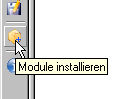
\includegraphics{ModuleInstall.png}
		\caption{PPTLC - Module Installieren}
		\label{fig:ModuleInstall}
	\end{figure}
	
	Klicken sie links im ToolBar auf das Paket-Symbol (siehe Abbildung 
	\ref{fig:ModuleInstall}). Dann �ffnet sich ein Dialog, in dem sie eine Datei aus w�hlen
	sollen. Wechseln sie also in der Ordner, in den sie das Modularchiv entpackt haben.
	Dort befindet sich eine Datei mit dem Namen \texttt{Setup.idf}. In dieser Datei wird
	beschrieben, wie die Module zu intallieren sind. W�hlen sie also diese Datei aus. 
	Danach sollten die Module. Ger�te und Server automatisch installiert werden. 
	
	Sollte es zu Fehlern kommen, pr�fen sie bitte ob sie als Administrator angemeldet sind.
	
	
	